\begin{figure}
\hfill
\subfigure[Jedes Element in einer Antidiagonalen kann parallel berechnet
werden.]{%
  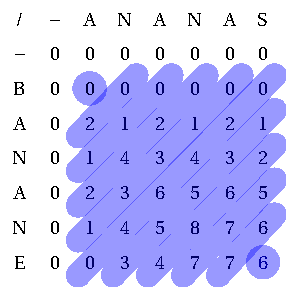
\includegraphics[width=.48\linewidth]{./img/sw_matrix/matrix_04.pdf}%
  \label{fig:anti}%
}
\hfill
\subfigure[Jede Submatrix kann pro Antidiagonale (grün, blau) parallel berechenet werden.]{%
  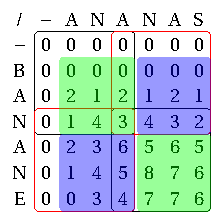
\includegraphics[width=.48\linewidth]{./img/sw_matrix/matrix_05.pdf}%
  \label{fig:sub}%
}
\hfill
\caption{Parallele Ausführung des Smith-Waterman Algorithmus mittels Antidiagonalen.
Antidiagonale müssen seriel berechnete werden. Jedoch sind ihre Element
voneinander unabhängig}
\end{figure}
